\documentclass[11pt,a4paper]{article}

% Stil-Datei laden
\usepackage{style/thesis}

% Metadaten
\title{From Differentiable Manifolds to Gauge Fields\\\large Von differenzierbaren Mannigfaltigkeiten zu Eichfeldern}
\author{Jonas von Stein}
\date{\today}

\begin{document}

% Titelblatt ENGLISCH
\selectlanguage{english}
\begin{titlepage}
    \centering
    {\LARGE Bachelor Thesis \par}
    \vspace{2cm}
    {\Huge \bfseries From Differentiable Manifolds to Gauge Fields \par}
    \vspace{1.5cm}
    {\Large Jonas von Stein \par}
    \vfill
    \textit{Supervisor: Prof. Dr. Ivo Sachs}\\
    \textit{Arnold Sommerfeld Center for Theoretical Physics \\ Ludwig-Maximilians-Universität Munich}\\
    \vspace{1cm}
    {\large \today\par}
\end{titlepage}

% Titelblatt DEUTSCH
\selectlanguage{ngerman}
\begin{titlepage}
    \centering
    {\LARGE Bachelorarbeit \par}
    \vspace{2cm}
    {\Huge \bfseries Von differenzierbaren Mannigfaltigkeiten zu Eichfeldern \par}
    \vspace{1.5cm}
    {\Large Jonas von Stein \par}
    \vfill
    \textit{Betreuer: Prof. Dr. Ivo Sachs}\\
    \textit{Arnold Sommerfeld Center for Theoretical Physics \\ Ludwig-Maximilians-Universität Munich}\\
    \vspace{1cm}
    {\large \today\par}
\end{titlepage}

% Inhaltsverzeichnis
\tableofcontents
\newpage

% Kapitel einbinden
\chapter{Introduction}

Differential geometry plays a central role in the formulation of modern physics. Many physical theories, notably gauge theories and general relativity, are naturally expressed on smooth manifolds equipped with geometric structures such as tensors, connections, and curvature. These mathematical tools provide a coordinate-independent framework in which physical laws can be formulated and understood. In the 20th century Wu and Yang formalized the idea that gauge fields, such as those describing electromagnetism or the strong and weak nuclear forces, can be understood as connections on principal bundles\cite{WuConceptnonintegrablephasefactorsglobalformulationgaugefields1975}, building on the work of Charles Ehreshmann. In this context, the curvature of a connection corresponds directly to the physical field strength, while gauge transformations are interpreted as changes of local trivialization. This geometric formulation reveals the profound mathematical structure behind gauge invariance and highlights the important role of symmetry in physics. The goal of this thesis is to elucidate how such geometric structures naturally lead to gauge fields. Starting from the definition of differentiable manifolds, more refined concepts are introduced—vector bundles, principal bundles, and connections—culminating in a complete formulation of classical gauge theory within the framework of differential geometry. Throughout, the focus remains on building the theory in a mathematically consistent manner. 

\textbf{Structure}

This thesis develops the geometric foundations of gauge theories by tracing a path from differentiable manifolds to fiber bundles, connections, and curvature. Starting with manifolds, tangent spaces, and bundles, the necessary tools from topology and geometry are introduced. Building on this, principal bundles and their connections are defined, leading to a geometric formulation of gauge fields as connection forms and their curvature as the field strength. Finally, classical gauge theories used in standard model physics are reintroduced within this framework, illustrating the reinterpretation of gauge fields as geometric objects.

\textbf{Objective}

The primary objective is to demonstrate how the mathematical concept of a connection on a principal bundle provides a natural and rigorous formulation of gauge fields. This approach underscores that many features of physical theories, such as field strength and gauge invariance, are consequences of the underlying geometric structure.
This thesis is concerned with the classical, differential-geometric formulation of gauge fields. Quantum aspects, topological phenomena, and the coupling of gauge fields to matter are not treated. The emphasis lies on comprehending the mathematical structure underlying gauge invariance and field strength in a coordinate-free way from a purely geometric perspective. Also, the theory of Lie groups will not be introduced, still some definitions will be provided. Underlying concepts can be found in sources used throughout this theses such as \cite{RaghunathanLieGroupsLieAlgebras2025} and \cite{NakaharaGeometrytopologyphysics2005}

\chapter{Manifolds}

Manifolds are the fundamental spaces used in physics. They provide a framework to describe topological spaces that locally resemble Euclidean spaces, allowing for the application of known methods from calculus and linear algebra.

\section{Preliminaries from topology}

Although this thesis will not focus on introducing topology, a few important results will be given here, which are necessary to understand the definition of manifolds. The following definitions and theorems are taken from \cite{NakaharaGeometrytopologyphysics2005}

A \textbf{topological space} is a set \( X \) equipped with a collection of open sets \( \mathcal{T} = \{ U_i \mid i\in I\} \) such that:
\begin{itemize}
    \item \( \emptyset, X \in \mathcal{T} \)
    \item For any subcollection $J$ of $I$ the Union of corresponding open sets is itself an open set \( \bigcup_{j\in J} U_j \in \mathcal{T} \)
    \item For any finite subcollection $K$ of $I$ the intersection of the corresponding open sets is open: \( \cap_{k \in K} U_k \in \mathcal{T} \)
\end{itemize}

A family $\{O_i\}$ of (open) subsets of $X$ is called an (open) covering of $X$ if \( X = \bigcup_i O_i \).

A subset $N$ is called a \textbf{neighborhood} of a point \( p \in X \) if there exists at least one open set \( U \in \mathcal{T} \) such that \( p \in U \subset N \). A topological space is called \textbf{Hausdorff} if for any two distinct points \( p, q \in X \) there exist neighborhoods \( N_p, N_q \) such that \( N_p \cap N_q = \emptyset \).

A map \( f: X \to Y \) between two topological spaces is called \textbf{continuous} if for every open set \( V \subset Y \) the preimage \( f^{-1}(V) \) is an open set in \( X \). If the inverse \( f^{-1} : Y \to X \) is also continuous, then \( f \) is called a \textbf{homeomorphism}. Two topological spaces are called \textbf{homeomorphic} if there exists a homeomorphism between them.

\section{Differentiable Manifolds}

A Hausdorff topological space $(M,\mathcal{T})$ is called a \textbf{d-dimensional manifold} if there exists an open covering \( \{U_i\} \) and a family of homeomorphisms \( \varphi_i: U_i \to \varphi_i(U_i) \subset \mathbb{R}^d \). The pair \( (U_i, \varphi_i) \) is called a \textbf{chart} and the family $\{(U_i,\varphi_i)\}$ is called an \textbf{atlas}\cite{FredericSchullerTopologicalmanifoldsmanifoldbundlesLec06FredericSchuller2015}.

$M$ is a \textbf{differentiable or smooth manifold} if for any $U_i$ and $U_j$ given that $U_i\cap U_j \neq \emptyset$ the transition function $\varphi_i \circ \varphi_j^{-1}: \varphi_j(U_j \cap U_i) \to \varphi_i(U_j \cap U_i)$ is infinite differentiable ($C^\infty$)\cite{NakaharaGeometrytopologyphysics2005}. In this thesis, smoothness will always be assumed, unless stated otherwise.

Let $M$ and $N$ be two differentiable manifolds of dimension $m$ and $n$ equipped with atlases $\{(U_i, \varphi_i)\}$ and $\{(V_j, \psi_j)\}$ respectively. A map \( f: M \to N \) is called a \textbf{differentiable map} at a point $p \in M$ if for $p \in U_i$ and $f(p) \in V_j$ the composition \( \psi_j \circ f \circ \varphi_i^{-1} : \varphi_i(U_i) \to \psi_j(V_j) \) is infinite differentiable. If $f$ is also a homeomorphism and the inverse \( f^{-1} : N \to M \) is differentiable, then $f$ is called a \textbf{diffeomorphism}. $M$ and $N$ are called \textbf{diffeomorphic} if there exists a diffeomorphism between them. This will be denoted as \( M \cong N \).


\section{Spacetime Manifold $M$}\label{sec:spacetime-manifold}

A trivial but for obvious reasons important example of a differentiable manifold is the spacetime manifold $M$ used in physics, which is defined as follows:

Let $M := \mathbb{R}^4$, the set of ordered 4-tuples $(x^\mu) \in \mathbb{R}^4$. The so called \textbf{standard topology} is defined by the open balls around a point $p \in M$ with radius $r > 0$:
\[
B_r(p) := \{ x \in \mathbb{R}^4 \mid \|x - p\| < r \}
\]
with $\| \cdot \|$ the Euclidean norm:
\[
\|x\|^2 = \sum_{\mu=0}^3 (x^\mu)^2
\]
This is obviously a Hausdorff\footnote{For two distinct points $p,q \in M$ it is always sufficient to choose $r=\frac12\|q - p\|$}, and locally Euclidean topological space. The identity map $\phi(p)=p$ covers $M$ globally. Hence, $(\mathcal{M}, B_r(p), \varphi)$ is a smooth manifold.


\chapter{Bundles}

  The definition of a vector on a Manifold is non-trivial because a vector space structure might not exist globally on the manifold. A Manifold may still be equipped with a Vector space structure locally. Thus, tangent spaces are introduced pointwise. Combining these local structures will lead naturally to the definition of fiber bundles.

\section{Tangent Space $T_pM$}

  Let $M$ be an $n$-dimensional smooth manifold. A tangent vector at a point $p \in M$ is a linear map $v: C^\infty(M) \to \mathbb{R}$ satisfying the Leibniz rule \cite{FredericSchullerDifferentialstructurespivotalconcepttangentvectorspacesLec09FredericSchuller2015}:
 \[ v[fg] = v[f]g(p) + f(p)v[g] \]

  A tangent vector at a point $p \in M$ can be constructed as the directional derivatives of an equivalence class of curves through $p$\cite{NakaharaGeometrytopologyphysics2005}.

  Let $\gamma: [-\epsilon, \epsilon] \to M$ be a smooth curve in $M$ with $\gamma(0)=p$. Then $\phi \circ \gamma(t) = x(t) \in \mathbb{R}^n$ is called the coordinate representation of $\gamma$ induced by a chart $(U, \varphi)$.
Let $f \in C^\infty(M)$ be a smooth function on $M$. The directional derivative of $f$ along the curve $\gamma$ at $t=0$ is given by:
\begin{align*}
\left. \frac{d}{dt} (f \circ \gamma)(t) \right|_{t=0}
  &= \left. \frac{d}{dt} \left( f\circ \varphi^{-1}\circ\varphi\circ\gamma(t) \right) \right|_{t=0} \\[0.8em]
&= \left. \frac{\partial f}{\partial x^r} \frac{d x^r}{dt} \right|_{t=0} \\[0.8em]
&= \left. \frac{d x^r}{dt} \right|_{t=0} \left. \frac{\partial f}{\partial x^r} \right|_p
\end{align*}

The definition of a tangent vector is now obtained by introducing an equivalence relation on curves. Two curves $\gamma_1$ and $\gamma_2$ are called equivalent at $\gamma_1(0)=\gamma_2(0)=p$ if their derivatives at $t=0$ are equal:
\[
\left. \frac{d x_1^r}{dt} \right|_{t=0}
= \left. \frac{d x_2^r}{dt} \right|_{t=0}
= v^r
\]
A tangent vector is identified with the differential operator given the equivalence class of curves. Once a chart $(U, \varphi)$ is chosen, with local coordinates $(x^1, \dots, x^n)$, a tangent vector is represented as a linear combination of partial derivatives with real coefficients.
\[
v = v^r \left. \frac{\partial}{\partial x^r} \right|_p
\]
The tangent space at a point $p \in M$ is then defined as the set of all tangent vectors at $p$ and is denoted by $T_pM$.
\[
\left\{ \left. \frac{\partial}{\partial x^1} \right|_p, \dots, \left. \frac{\partial}{\partial x^n} \right|_p \right\} \quad \text{form a basis of } T_pM
\]



\section{The Tangent Bundle as a Fiber Bundle}

To introduce the concept of fiber bundles, a detailed examination of a specific example, the tangent bundle, serves as an effective foundation.
The tangent bundle of a smooth \( n \)-dimensional manifold \( M \) is constructed by taking the disjoint union of all tangent spaces \( T_pM \). This construction can be represented as:
\[
TM := \bigsqcup_{p \in M} T_pM = \bigcup_{p \in M} \{p\} \times T_pM
\]
Here, \( T_pM \) denotes the tangent space at a point \( p \in M \). The tangent space \( T_pM \) is a vector space that consists of all tangent vectors at the point \( p \). It should be noted that this notation emphasizes the pointwise nature of the disjoint union, where each tangent space is associated with a specific point on the manifold. Since each tangent space is a different object, a certain tangent vector in a tangent space can only belong to that specific tangent space. Therefore all the information is already in the vector itself and the direct product notation \( \{p\} \times T_pM \) is only used to clarify \cite{FredericSchullerTopologicalmanifoldsmanifoldbundlesLec06FredericSchuller2015}.

Each element of the tangent bundle \( TM \) can be expressed as a pair \( (p, v) \), where \( p \) is a point on the manifold \( M \), and \( v \) is a tangent vector belonging to the tangent space \( T_pM \) at that point. 
A natural projection map is defined as follows:
\[
\pi: TM \to M, \quad (p, v) \mapsto p
\]
This projection, \( \pi \), serves to "forget" the tangent vector \( v \) associated with each point, effectively collapsing all the tangent vectors at \( p \) to the single point \( p \) in the base manifold \cite{NakaharaGeometrytopologyphysics2005}.

The fiber over a point \( p \) is denoted as \( \pi^{-1}(p) = T_pM \). This represents all the tangent vectors at the point \( p \). Since \( T_pM \) is isomorphic to \( \mathbb{R}^n \) as a vector space, it is referred to as the model fiber, denoted \( F = \mathbb{R}^n \) \cite{NakaharaGeometrytopologyphysics2005}.
Since the fiber of the tangent bundle is a vector space, the tangent bundle is also referred to as a \textbf{vector bundle}.

Consider a coordinate chart \( (U, \varphi) \) on \( M \). The chart \( \varphi \) provides a mapping from an open set \( U \subseteq M \) to an open subset of \( \mathbb{R}^n \). A diffeomorphism on the preimage \( \pi^{-1}(U) \subset TM \) can then be defined as:
\[
\Psi: \pi^{-1}(U) \to \mathbb{R}^{2n}, \quad (p, v) \mapsto \left(x^1(p), \dots, x^n(p), v^1, \dots, v^n \right)
\]
where the coordinates \( x^i(p) \) represent the local coordinates of the point \( p \) in \( U \), and \( v = v^i \left. \frac{\partial}{\partial x^i} \right|_p \) describes the tangent vector in terms of its components in the chosen coordinate system \cite{NakaharaGeometrytopologyphysics2005}.
This establishes a local trivialization of the tangent bundle, expressed as:
\[
TM|_U \cong U \times \mathbb{R}^n
\]

In summary, the construction of the tangent bundle yields a fiber bundle characterized by the following essential components:
\begin{itemize}
  \item \textbf{Total space:} \( TM = \bigsqcup_{p \in M} T_pM \), encapsulating all tangent spaces.
  \item \textbf{Base space:} \( M \), a manifold to which additional structure is added.
  \item \textbf{Projection:} \( \pi: TM \to M \), mapping each tangent vector to its associated point on the manifold.
  \item \textbf{Model fiber:} \( F = \mathbb{R}^n \), serving as the standard fiber structure over each point.
  \item \textbf{Local trivialization:} \( TM|_U \cong U \times \mathbb{R}^n \), ensuring that the tangent bundle locally resembles a product structure.
\end{itemize}

 Similar to the way a manifold is commonly perceived as a space that locally resembles \( \mathbb{R}^n \), a fiber bundle may be conceptualized as a space that locally resembles the Cartesian product of the base space with a typical fiber structure. 


\section{Definition of a Fiber Bundle}

The formal definition of a fiber bundle reads as follows\cite{FredericSchullerTopologicalmanifoldsmanifoldbundlesLec06FredericSchuller2015, DudekEhreshmanntheoryconnectionprincipalbundlecompendiumphysicists2018}.
A fiber bundle is a quadruple $(E, B, \pi, F)$ where:
\begin{itemize}
  \item $E$ is the total space
  \item $B$ is the base space
  \item $\pi: E \to B$ is a surjective map called the projection
  \item $F$ is the typical fiber
\end{itemize}

There exists an open cover $\{U_\alpha\}$ of $B$ such that for each $\alpha$, there is a diffeomorphism
\[
\varphi_\alpha: \pi^{-1}(U_\alpha) \to U_\alpha \times F
\]
such that the following diagram commutes:


\begin{center}
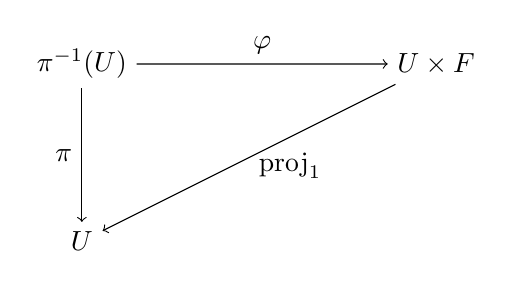
\begin{tikzpicture}[scale=1.5, every node/.style={font=\normalsize}]
  \node (A) at (0,1.5) {$\pi^{-1}(U)$};
  \node (B) at (3,1.5) {$U \times F$};
  \node (C) at (0,0) {$U$};

  \draw[->] (A) -- (B) node[midway, above] {$\varphi$};
  \draw[->] (A) -- (C) node[midway, left] {$\pi$};
  \draw[->] (B) -- (C) node[midway, right, yshift=-3pt] {$\mathrm{proj}_1$};
\end{tikzpicture}
\end{center}


where $\text{proj}_1: A \times B \to A$ is the first projection. $(U_\alpha, \varphi_\alpha)$ are called \emph{local trivialization}. The fiber over a point $b \in B$ is:
\[
F_b := \pi^{-1}(\{b\}) \cong F
\]

Often the notations $E \xrightarrow{\pi} B$ or $\pi : E \to B$ are used to denote a fiber bundle.


\subsection{The Structure Group of a Fiber Bundle}

Above a fiber bundle was defined as a quadruple \((E, B, \pi, F)\) equipped with local trivializations. These local trivializations are established as diffeomorphisms on an open cover $\{U_\alpha\}$ of the base space \(B\). The definition does not impose the requirement that \(U_\alpha \cap U_\beta = \emptyset\). For a point \(p \in U_\alpha \cap U_\beta\), multiple local trivializations \(\varphi_\alpha(p, f) = \varphi_{\alpha,p}(f)\) and \(\varphi_\beta(p, f) = \varphi_{\beta,p}(f)\) may be present, defined on \(U_\alpha\) and \(U_\beta\), respectively.

The \textbf{structure group} \(G\) of a fiber bundle is defined as the Lie group of diffeomorphisms relating these local trivializations. The corresponding transition function is given by\cite{NakaharaGeometrytopologyphysics2005}:

\[
t_{\alpha\beta}(p) \equiv \varphi_{\alpha,p}^{-1} \circ \varphi_{\beta,p} : F \to F
\]

This establishes a smooth map \(t_{\alpha\beta}: U_\alpha \cap U_\beta \to G\) that satisfies the following properties:

\begin{align*}
  t_{\alpha \alpha}(p) &= \mathrm{id}_F && \forall\, p \in U_\alpha \\
  t_{\alpha\beta}(p) &= t_{\beta\alpha}(p)^{-1} && \forall\, p \in U_\alpha \cap U_\beta \\
  t_{\alpha\beta}(p) \circ t_{\beta\gamma}(p) &= t_{\alpha\gamma}(p) && \forall\, p \in U_\alpha \cap U_\beta \cap U_\gamma
\end{align*}

In the case of the tangent bundle, the structure group corresponds to the general linear group \(\mathrm{GL}(n, \mathbb{R})\), which consists of all invertible \(n \times n\) matrices. 
A fiber bundle where all transition maps can be chosen to be the identity map is termed a \textbf{trivial bundle}. In this scenario, the total space \(E\) is diffeomorphic to the product space \(B \times F\). 

Generally, a fiber bundle does not possess a unique trivialization. Let \(\{\varphi_\alpha\}\) and \(\{\tilde{\varphi}_\alpha\}\) denote two local trivializations over the same open covering that describe the same fiber bundle. These trivializations are related by maps \(g_\alpha(p) : F \to F \quad \forall\, p \in B\), where each \(g_\alpha(p)\) is a homeomorphism within the structure group \(G\). The transition function between the two local trivializations is then given by:

\[
g_\alpha(p) \equiv \varphi_{\alpha,p}^{-1} \circ \tilde{\varphi}_{\alpha,p}
\]

Considering the tangent bundle as an illustrative example\cite{NakaharaGeometrytopologyphysics2005}, let \(U_i\) and \(U_j\) represent overlapping charts with \(p \in U_i \cap U_j\). Utilizing the basis \(\left\{ \left. \frac{\partial}{\partial x^i} \right|_p \right\}\) and \(\left\{ \left. \frac{\partial}{\partial y^j} \right|_p \right\}\), a vector \(v \in T_pM\) can be expressed in both bases as:

\[
v = v^{\mu} \frac{\partial}{\partial x^{\mu}} = \tilde{v}^{\mu} \frac{\partial}{\partial y^{\mu}}
\]

The transition function \(t^\nu_{\,\,\mu}\) is thus defined as:

\[
\tilde{v}^\nu = \left.\frac{\partial y^\nu}{\partial x^\mu}\right|_p v^\mu = t^\nu_{\,\,\mu} v^\mu
\]

\subsection{Sections}

An important definition in the context of fiber bundles is that of a section or cross-section. This concept enables the selection of an element from each fiber over each point in a continuous manner, facilitating the introduction of ideas such as vector fields over spacetime\cite{NakaharaGeometrytopologyphysics2005}.

A \textbf{section} of a fiber bundle \(\pi : E \to B\) is defined as a continuous map \(s: B \to E\) such that

\[
\pi \circ s = \mathrm{id}_B.
\]

This condition ensures that exactly one point is chosen from each fiber continuously. 
The set of all (smooth) sections is denoted by:
\[
\Gamma(E) := \left\{ s: M \to E \mid \pi \circ s = \mathrm{id}_{M} \right\}.
\]
It is also possible to define a section locally on an open set \(U \subset B\) as a map \(s: U \to E\) such that \(\pi \circ s = \mathrm{id}_U\). In this case, the section is called a \textbf{local section}.
For example, a vector field over a manifold $M$ can therefore be understood as a section of the tangent bundle \(TM\) over \(M\).

\section{The cotangent bundle and differential forms}

\subsection{The Cotangent Bundle}
In this section the fundamental concepts of the cotangent bundle are introduced, which is essential for the definition of differential forms and the exterior derivative. The cotangent space at a point $p$ on a manifold $M$ is defined as the dual space of the tangent space at that point. Formally, the cotangent space at a point $p \in M$ is the set of all linear maps from the tangent space at that point to the real numbers\cite{NakaharaGeometrytopologyphysics2005}.
\[
T_p^*M := \text{Hom}_\mathbb{R}(T_p M, \mathbb{R})
\]
A covector \(\omega \in T_p^*M\) is such a linear function:
\[
\omega: T_p M \to \mathbb{R}
\]
As an example, consider a function \(f \in C^\infty(M)\) and some tangent vector $v \in T_pM$. Then $v[f] \in \mathbb{R}$ by definition. The differential of \(f\) at a point \(p\) is a covector $df_p$ and therefore $df_p[v]\in \mathbb{R}$ is simply defined as $df_p[v] = v[f]$.
Given a coordinate basis \(\left\{ \left. \frac{\partial}{\partial x^i} \right|_p \right\}\)  of \(T_p M\) the dual basis is:
\[
\left\{ \left. dx^i \right|_p \right\}
\]
satisfying the relation:
\[
dx^i\left( \left. \frac{\partial}{\partial x^j} \right|_p \right) = \delta^i_j
\]
The example from before can thus be expressed as:
\[
df_p = \frac{\partial f}{\partial x^i} dx^i \quad \text{and} \quad df_p[v] = v^i \left. \frac{\partial f}{\partial x^i} \right|_p
\]
Analogous to the tangent bundle, the cotangent bundle is defined as the disjoint union of all cotangent spaces at each point in the manifold:
\[
T^*M := \bigsqcup_{p \in M} T_p^* M
\]
This structure constitutes a vector bundle over \(M\). A section of the cotangent bundle can be defined as:
\[
\omega \in \Gamma(T^* M)
\]
This section assigns to each \(p \in M\) a covector \(\omega_p \in T_p^*M\) smoothly. Such a section is referred to as a \textbf{1-form}. In a coordinate representation, a 1-form can be expressed as:
\[
\omega = \sum_{i=1}^n \omega_i(x) \, dx^i
\quad \text{with} \quad \omega_i \in C^\infty(M)
\]

\subsection{Tensor Fields and the Metric Tensor}

Utilizing the fact that the fibers of the cotangent bundle are vector spaces, tensor products of bundles can be defined. For instance:
\[
T^*M \otimes T^*M := \bigsqcup_{p \in M} T_p^*M \otimes T_p^*M
\]
This forms a bundle whose fibers consist of maps form $TM \otimes TM$ to $\mathbb{R}$. Sections of this bundle are referred to as \((0,2)\)-tensor fields. A prominent example of such fields is the metric tensor. The Minkowski metric is defined as:
\[
\eta \in \Gamma(T^*M \otimes T^*M)
\]
In local coordinates, the Minkowski metric can be expressed as:
\[
\eta = \eta_{\mu\nu} \, dx^\mu \otimes dx^\nu
\quad \text{with} \quad \eta_{\mu\nu} = \text{diag}(1, -1, -1, -1)
\]
In general, a tensor field of type $(i,j)$ is a section of the bundle \cite{NakaharaGeometrytopologyphysics2005}:
\[ \otimes^iT^*M \otimes^jTM \]


\subsection{Differential Forms and the Exterior Derivative}
A \textbf{k-form} or \textbf{differential form} of order k is a totally antisymmetric $(k,0)$ tensor. To define a k-form, it is necessary to take the \textbf{wedge product} of 1-forms, which is defined by taking the totally antisymmetrized tensor product of 1-forms. This means that all permutations of the tensor product are considered, with even permutations contributing positively and odd permutations contributing negatively. Consider the cotangent space $T_p^*M$ of a manifold $M$ at a point $p$ with basis $\{dx^\mu\}$. The wedge product of two 1-forms \(dx^\mu\) and \(dx^\nu\) thus reads:
\[
dx^\mu \wedge dx^\nu = dx^\mu \otimes dx^\nu - dx^\nu \otimes dx^\mu
\]
Higher order forms can be constructed analogously. By taking the cotangent bundle \(T^*M\) and considering the antisymmetrized tensor product, we can define fields of differential forms of order \(r\) as:
\[\Omega^r(M) \equiv \Gamma(\wedge^r (T^*M))\]

The \textbf{exterior derivative} is then defined as a map \cite{NakaharaGeometrytopologyphysics2005}:
\begin{align*}
  d: \Omega^r(B) &\to \Omega^{r+1}(B) \\
  \omega &\mapsto d\omega = \frac{1}{r!}\left( \frac{\partial}{ \partial x^\nu} \omega_{\mu_1 \dots \mu_r} \right) dx^\nu \wedge dx^{\mu_1} \wedge \dots \wedge dx^{\mu_r}
\end{align*}

In the following, two relations will be shown that will be used in later proofs \cite{NakaharaGeometrytopologyphysics2005}. First consider the action of the exterior derivative on a 1-form $\omega=\omega_\mu dx^\mu \in \Omega^1(M)$ on two tangent vector fields $v=v^\mu\frac{\partial}{\partial x^\mu}$ and $w=w^\nu\frac{\partial}{\partial x^\nu}$:
\begin{align*}
  d\omega(V, W) 
  &= \left( \frac{\partial \omega_\mu}{\partial x^\nu} \, dx^\nu \wedge dx^\mu \right)(V, W) \\
  &= \frac{\partial \omega_\mu}{\partial x^\nu} 
  \left( dx^\nu(V) \, dx^\mu(W) - dx^\nu(W) \, dx^\mu(V) \right) \\
  &= \frac{\partial \omega_\mu}{\partial x^\nu} 
  \left( V^\nu W^\mu - W^\nu V^\mu \right) \\
  &= V^\nu \frac{\partial}{\partial x^\nu} \left( \omega_\mu W^\mu \right)
  - W^\nu \frac{\partial}{\partial x^\nu} \left( \omega_\mu V^\mu \right)
  - \omega_\mu \left( V^\nu \frac{\partial W^\mu}{\partial x^\nu} - W^\nu \frac{\partial V^\mu}{\partial x^\nu} \right) \\
  &= V[\omega(W)] - W[\omega(V)] - \omega([V, W])
\end{align*}
This gives a coordinate free expression for the action of the exterior derivative of a 1-form. Furthermore, it can easily be shown that the exterior derivative of a exterior derivative is zero, by using the fact that the product of a symmetric and an antisymmetric tensor is zero. By definition the following is obtained:
\[ d^2\omega = \frac{1}{r!}\left( \frac{\partial^2}{ \partial x^\alpha x^\beta} \omega_{\mu_1 \dots \mu_r} \right) dx^\alpha \wedge dx^\beta \wedge dx^{\mu_1} \wedge \dots \wedge dx^{\mu_r} \]
From this it follows instantly that $d^2=0$ since $\frac{\partial^2}{ \partial x^\alpha x^\beta}$ is symmetric and the wedge product is antisymmetric.




\chapter{Principal Bundles}

A principal bundle is a fiber bundle $P \xrightarrow{\pi} M$ is a bundle whose fiber is identical to the structure group. This framework is of particular importance, because it allows to understand fibre bundles with fibre $F$ on which $G$ acts. These bundles are called \emph{associated bundles} and are essential to understand Gauge theories in physics.

\section{Action of a Lie Group on a Manifold}\label{sec:action-of-lie-group-on-manifold}

To understand this properly we first need to understand how a Lie group $G$ can act on a manifold $M$ \cite{FredericSchullerPrincipalfibrebundlesLec19FredericSchuller2015}
Let \( (G, \cdot) \) be a Lie group, and \( M \) a smooth manifold.  
Then a smooth map
\[
\triangleright : G \times M \longrightarrow M
\]
satisfying
\begin{align*}
  e \triangleright p &= p && \forall p \in M, \text{ and $e$ being the identity in $G$} \\
  g_2 \triangleright (g_1 \triangleright p) &= (g_2 \cdot g_1) \triangleright p && \forall g_1, g_2 \in G, \, p \in M
\end{align*}
is called a \textbf{left \( G \)-action} on \( M \).

Analogous a \textbf{right \( G \)-action} $\triangleleft : M \times G \longrightarrow M$ is defined, satisfying:
\begin{align*}
p \triangleleft e &= p && \forall p \in M, \text{ and $e$ being the identity in $G$} \\
  (p \triangleleft g_1) \triangleleft g_2 &= p \triangleleft (g_1 g_2) && \forall g_1, g_2 \in G, \, p \in M
\end{align*}

Given a left action $\triangleright$, we can construct a right action: 
\begin{align*}
  \triangleleft : &M \times G \longrightarrow M, \\
  & p \triangleleft g := g^{-1} \triangleright p.
\end{align*}

It is trivial to show that this yields a right action.

Let \( G \) be a Lie group acting smoothly on a manifold \( M \) from the left via
\[
\triangleright : G \times M \longrightarrow M.
\]

We define an equivalence relation \( \sim \) on \( M \) by:

\begin{align*}
p \sim \tilde{p} \quad :\Longleftrightarrow \quad \exists g \in G \text{ such that } \tilde{p} = g \triangleright p.
\end{align*}

This defines an equivalence relation:
\begin{itemize}
  \item \textbf{Reflexivity:} \( e \triangleright p = p \), so \( p \sim p \).
  \item \textbf{Symmetry:} If \( \tilde{p} = g \triangleright p \), then \( p = g^{-1} \triangleright \tilde{p} \), so \( \tilde{p} \sim p \).
  \item \textbf{Transitivity:} If \( \tilde{p} = g_1 \triangleright p \) and \( \hat{p} = g_2 \triangleright \tilde{p} \), then
  \[
  \hat{p} = g_2 \triangleright (g_1 \triangleright p) = (g_2 g_1) \triangleright p,
  \]
  so \( p \sim \hat{p} \).
\end{itemize}

The \textbf{orbit} of a point \( p \in M \) under the group action is then the equivalence class:
\[
\mathcal{O}_p := \{ \tilde{p} \in M \mid \exists g \in G : \tilde{p} = g \triangleright p \}.
\]

We can then define the \textbf{quotient space} \( M/\!\sim \), often denoted \( M/G \), by identifyinf points that are in the same orbit.

We define the \textbf{stabilizer} of a point \( p \in M \) as the set of elements in \( G \) that leave \( p \) unchanged:
\[ S_p \coloneqq \{g \in G \mid g \triangleright p = p \} \]

An action $\triangleright$ is called free if for all \( p \in M \) the stabilizer is trivial \( S_p = \{e\} \).





\section{Principal Bundles}

We now define a principal fibre bundle as follows \cite{FredericSchullerPrincipalfibrebundlesLec19FredericSchuller2015} 

Let \( (P, \pi, M, F) \) be a fibre bundle. If the following conditions are satisfied, we call it a \textbf{principal \( G \)-bundle}:

\begin{align*}
  \text{(i)}\quad & P \text{ is equipped with a right } G\text{-action } \triangleleft, \\
  \text{(ii)}\quad & \text{The action of } G \text{ is free}, \\
  \text{(iii)}\quad & \pi : P \to M \text{ is isomorphic as a bundle to the quotient } \rho : P \to P/G,
\end{align*}

where \( \rho(p) \mapsto [p] \) denotes the canonical projection onto the orbit space \( P/G \). 

To clarify, two bundles \( \pi: E \to M \) and \( \pi': E' \to M' \) are isomorphic if there exist diffeomorphisms \( \bar{f}: E \to E' \) and \( f: M \to M' \) such that \( \pi' \circ \bar{f} = f \circ \pi \).

Since \( \triangleleft \) acts freely, each fibre \( \rho^{-1}([p]) \) is diffeomorphic to \(G\).


\paragraph{The Frame Bundle}

As an example we consider the frame bundle of a smooth manifold \( M \).

We define a \textbf{frame} at a point \(p\in M\) with \(\text{dim} M = d\) as an ordered basis of the tangent space \(T_pM\) and the set  of all frames at \(p\) as:
\[
L_pM \coloneqq \left\{ (e_1, \dots, e_d) \,\middle|\, \{e_1, \dots, e_d\} \text{ is a basis of } T_pM \right\}
\]

There exists a natural isomorphism
\[
L_pM \cong \mathrm{GL}(d, \mathbb{R}),
\]
by identifying each frame \( (e_1, \dots, e_d) \in L_pM \) with the matrix whose columns are the components of the vectors \( e_i \). Concretely, each frame is mapped to a matrix \( g \in \mathrm{GL}(d, \mathbb{R}) \) such that
\[
g^\mu_{\;\;\alpha} = e^\mu_{\;\;\alpha}
\]



Analogous to the tangent bundle, we can define the \textbf{frame bundle}:
\[ LM := \bigsqcup_{p \in M} L_pM \]

Given a chart \(U_i\) on \( M \), we can define a local trivialization of the frame bundle \cite{NakaharaGeometrytopologyphysics2005}. A frame $\epsilon = \{e_1, \dots, e_d\}$ at $p\in M$ is expressed in terms of the natural basis of the tangent space \(T_pM\) \( \left\{ \partial / \partial x^\mu \mid_p \right\} \)
\[ e_\alpha = e^\mu_{\,\,\alpha} \, \partial/\partial x^\mu \mid_p \quad \text{where }e^\mu_{\,\,\alpha} \in \mathrm{GL}(d, \mathbb{R}) \]
The local trivialization is then given by \( \varphi_i^{-1}(u)=(p,(e^\mu_{\,\,\alpha}))\).

The projection $\pi_L$ of a frame $\epsilon = \{e_1, \cdot, e_d\}$ at a point \(p\in M\) is given by:
\begin{align*}
  \pi_L \, : \, LM &\longrightarrow M, \\
        \epsilon &\mapsto \pi_L(\epsilon)=p
\end{align*}

Therefore we have introduced the necessary structure, suck that $(LM, \pi, M, \text{GL}(d,\mathrm{R})$ defines a fiber bundle. 

The right action of \( \mathrm{GL}(d,\mathbb{R}) \) on the frame is defined as we would expect, since it is analogguss to the change of basis in a vector space:
\begin{align*}
  \triangleleft : LM \times \mathrm{GL}(d,\mathbb{R}) &\longrightarrow LM, \\
  (\epsilon, g) &\mapsto \epsilon \triangleleft g = (e_1, \cdots, e_d) \triangleleft g = (e_i g^i_{\,\,1}, \cdots, e_i g^i_{\,\,d}),
\end{align*}

To show that this Bundle equipped with this right action is a principal bundle, we need to check, if the action is free and the bundle is isomorphic to the quotient bundle.

Therefore we need to show that \( e_i g^i_{\,\,\alpha} = e_\alpha \implies g^i_{\,\,\alpha} = \delta^i_{\,\,\alpha} \, \forall \alpha \) . Since \( \{e_1, \dots, e_d\} \) is a basis, they are linearly independent. Therefore the definition already implies that \( g^i_{\,\,\alpha} = \delta^i_{\,\,\alpha} \) and thus the action is free.

To show the second condition, we need to show that the orbit space \( LM/\mathrm{GL}(d,\mathbb{R}) \) is consists of a single point for each \( \epsilon \in \pi^{-1}(p) \). This is indeed the case, since the orbit of a frame at \( p \in M \) under the action of \( \mathrm{GL}(d,\mathbb{R}) \) consists of all frames at \( p \), since the action is transitiv. Thus the quotient space is diffeomorphic to \( M \), with the diffeomorphism being: \( f: M \longrightarrow LM/\mathrm{GL}(d, \mathbb{R}), \, p \mapsto [\epsilon] \) where \( \epsilon \) is a frame at \( p \).




\chapter{Connections on Principal Bundles}

\section{General Definition}

A Connection is a consistent way to separate the tangent space of a principal bundle into a vertical subspace tangent to the fiber and a horizontal subspace that complements the former. This will be constructed by considering a vector field generated by the right action of the one-parameter subgroup of the structure group $G$ on the principal bundle. As before a vector is defined by its action on a function evaluated along a curve which will be generated by the former mentioned right action.

Let \( P \xrightarrow{\pi} M \) be a principal bundle with structure group \( G \). The right action of \( G \) on \( P \) induces a vector field as follows: For each \( A \in \mathfrak{g} \cong T_eG \), the action of the one-parameter subgroup \( \exp(tA) \) on an element \( p \in P \) yields a curve. Since the group acts within the fiber, it holds that \( \pi(p) = \pi(p \triangleleft \exp(tA)) = p \). A vector \( X^A_p \in T_pP \) is defined by its action on a function \( f \in C^\infty(P) \) \cite{NakaharaGeometrytopologyphysics2005}:

\[
X^A_p f = \frac{d}{dt} f(p \triangleleft \exp(tA))\mid_{t=0}.
\]

Furthermore, a vector space isomorphism \( i: \mathfrak{g} \longrightarrow \Gamma(TP) \) is defined that assigns to each element \( A \in \mathfrak{g} \) the vector field \( X^A \) which is generated by $A$. This vector field is referred to as a \textbf{fundamental vector field} on \( P \).

The \textbf{Pushforward} \cite{Pushforward2025} of a smooth map \( F:M \longrightarrow N \) between smooth manifolds \( M \) and \( N \) is defined as a map between the tangent spaces:
\[
F_* : T_pM \longrightarrow T_{F(p)}N.
\]
This is identified using \( (F_*v)(f) = v(f\circ F) \) for \( v \in T_pM \) and \( f \in C^\infty(N) \).

The pushforward of the projection map \( \pi_* : TP \longrightarrow TM \) facilitates the construction of the \textbf{vertical subspace} \( V_pP \coloneq \ker(\pi_*) \) at a point \( p \in P \), which serves as a vector subspace of the tangent space of \( P \).
It is noteworthy that each fundamental vector \( X^A_p \in V_pP \), since \( \pi_* (X^A_p) = 0 \) by construction.

A \textbf{connection} on a principal bundle \( P \xrightarrow{\pi} M \) is defined as a decomposition of the tangent space \( T_pP \) into a vertical subspace \( V_pP \) and a \textbf{horizontal subspace} \( H_pP \). This is achieved by choosing a complement to the vertical subspace at each point \( p \in P \) such that \cite{DudekEhreshmanntheoryconnectionprincipalbundlecompendiumphysicists2018}:
\newpage
\begin{enumerate}[label=(\roman*), labelsep=1em, leftmargin=2.5em]
  \item \( T_pP = H_pP \oplus V_pP \)

  \item \( (\triangleleft g)_*(H_pP) = H_{p \triangleleft g}P \quad \text{for all } g \in G \)

  \item For every smooth vector field \( X \in \Gamma(TP) \), the unique decomposition
  \( X = X^H + X^V \) with \( X^H(p) \in H_pP \) and \( X^V(p) \in V_pP \)
  produces smooth vector fields \( X^H \in \Gamma(HP) \), \( X^V \in \Gamma(VP) \).
\end{enumerate}

Condition (ii) ensures that when moving along the fibers via the action of \( G \), the horizontal subspace changes smoothly, while condition (iii) guarantees that the horizontal subspace varies smoothly when traversing the manifold \( P \).


\section{Connection One-Form}

The choice of a horizontal subspace at each point \( p \in P \) can be achieved by defining a Lie algebra-valued one-form. The horizontal subspace is then interpreted as the kernel of this one-form. The \textbf{connection one-form} \( \omega \in \mathfrak{g} \otimes T^*P \) is defined as a \( \mathfrak{g} \)-valued one-form on \( P \) such that:

\begin{align*}
  \text{(i)}\quad 
    & \omega(X^A) = A \quad \text{for all } A \in \mathfrak{g} \\
  \text{(ii)}\quad 
    & (\triangleleft g)^* \omega = \text{Ad}_{g^{-1*}} \omega \quad \text{for all } g \in G 
\end{align*}

Here, \( (\triangleleft g)^* \omega \) denotes the pullback of the connection one-form by the right action of \( g \in G \) on \( P \), and \( \text{Ad}_{g^{-1}} \) is the adjoint action of \( g^{-1} \) on the Lie Group \( G \). This implies that \( \omega_{p \triangleleft g}(X_p(\triangleleft g)_*) = g^{-1} \cdot_* \omega_p(X_p) \cdot_* g \). The horizontal subspace \( H_pP \) is then defined as the kernel of the connection one-form \cite{NakaharaGeometrytopologyphysics2005}
\[ H_pP \equiv \{ X \in T_pP \mid \omega(X)=0 \} \]

This is consistent with the general definition of a connection. The smoothness of the decomposition is guaranteed by the fact that the connection one-form is a section, which is smooth by definition. It is therefore sufficient to show that the horizontal subspace is invariant under the right action of \( G \).
To show this, consider a vector $X$ at a point $p \in P$ such that $X \in H_pP$. By definition $\omega(X) = 0$. For any element $g \in G$ the pushforward of the right action on $X$ can be acted on by $\omega$ \cite{NakaharaGeometrytopologyphysics2005}:
\[ \omega((\triangleleft g)_* X) = (\triangleleft g)^* \omega(X) = g^{-1} \cdot \omega(X) \cdot g = 0 \]
Therefore $(\triangleleft g)^* X$ is again a horizental vector at the point $p\triangleleft g$. Futhermore, any vector $\tilde{X} \in H_{p\triangleleft g}P$ can thus be obtained by the right action on some vector $X \in H_pP$. Therefore $ (\triangleleft g)_* (H_pP) = H_{p \triangleleft g}P $


\section{Local Connection Form}

The connection one-form, as defined above, is a global object on the principal bundle \( P \). However, in practice, it is often useful to work with local connection forms, which will be identified with the gauge potential in physical gauge theories.

Consider an open covering \( \{U_i\} \) of the base manifold \( M \) and local sections \( \sigma_i : U_i \rightarrow \pi^{-1}(U_i) \). A Lie-algebra valued one-form \( \mathcal{A}_i \equiv \sigma_i^* \omega \in \mathfrak{g} \otimes\Omega^1(U_i) \) is defined for a global connection one-form \( \omega \) \cite{NakaharaGeometrytopologyphysics2005}. This local connection form is termed a \textbf{Yang-Mills field} \cite{FredericSchullerLocalrepresentationsconnectionbasemanifoldYangMillsfieldsLec222015}.

Given a local section \( \sigma_i : U_i \to P \), a local trivialization is established:
\begin{align*}
  \psi_i : U_i \times G &\longrightarrow \pi^{-1}(U_i) \subset P \\
  (p, g) &\mapsto \sigma_i(p) \triangleleft g
\end{align*}

This trivialization introduces a local representation of the global connection one-form \( \omega \) via its pullback:

\begin{align*}
  \psi_i^* \omega : T_{(p, g)}(U_i \times G) &\longrightarrow \mathfrak{g} \\
  (\psi_i^* \omega)_{(p, g)}(X) &= \omega_{\sigma_i(p) \triangleleft g}\left((\psi_i)_* X\right)
\end{align*}

The relations of the above maps are illustrated in the following diagram:
\begin{figure}[h!]
  \centering
  \begin{tikzpicture}[scale=1.3, every node/.style={scale=1}]
    % Matrix for main layout
    \matrix (m) [matrix of math nodes, row sep=3.7em, column sep=4.7em, ampersand replacement=\&] {
    \& \& \\
    \& U_i \times G \& \pi^{-1}(U_i) \subset P \\
    \& U_i \& M \\
    \& \& \\
    };

    % Manually placed nodes for forms
    \node (omegaPsi) at ($(m-2-2) + (-1.2, 1)$) {\(\psi_i^* \omega\)};
    \node (omegaSigma) at ($(m-3-2) + (-1.2, -1)$) {\(\sigma_i^* \omega\)};

    % Solid arrows (maps)
    \path[->]
    (m-2-2) edge node[above] {\(\psi_i\)} (m-2-3)
    (m-3-2) edge node[left, yshift=0.5ex] {\(\sigma_i\)} (m-2-3)
    (m-3-2) edge node[below] {\(\text{id}\)} (m-3-3)
    (m-2-2) edge node[left] {\(\text{proj}_1\)} (m-3-2)
    (m-2-3) edge node[right] {\(\pi\)} (m-3-3);

    % Dashed arrows for associated forms
    \path[dashed,->]
    (omegaPsi) edge[out=-60, in=120] (m-2-2)
    (omegaSigma) edge[out=60, in=-120] (m-3-2);

  \end{tikzpicture}
  \caption{Local trivialization \(\psi_i\) and local connection forms \(\psi_i^*\omega\) and \(\sigma_i^*\omega\) associated to \(U_i \times G\) and \(U_i\), respectively.}
\end{figure}

This local representation is related to the Yang-Mills field \( \mathcal{A}_i \) by \cite{FredericSchullerLocalrepresentationsconnectionbasemanifoldYangMillsfieldsLec222015}:

\begin{align*}
  (\psi_i^* \omega)_{(p, g)}(X) &= \text{Ad}_{g^{-1*}} \left(\mathcal{A}_i (X)\right) + \Xi_g(X) \\
\end{align*}

Here, \( \Xi \) denotes the \textbf{Maurer–Cartan form} of the Lie group \( G \). This form takes a tangent vector \( v \in T_gG \) and maps it to the unique Lie algebra element (i.e., a tangent vector at the identity) that generates \( v \) via left translation:

\[
\Xi(v) = (g^{-1} \triangleright)_* v \in T_eG \cong \mathfrak{g}
\]

This formulation exploits the fact that every tangent vector on \( G \) arises as the pushforward of a unique element of the Lie algebra \( \mathfrak{g} = T_eG \) under left action \cite{RaghunathanLieGroupsLieAlgebras2025}. Thus, for every \( v \in T_gG \), there exists a unique \( X \in \mathfrak{g} \) such that

\[
v = (g \triangleright)_* X.
\]

Consequently, \( \Xi \) identifies the tangent bundle \( TG \) with \( G \times \mathfrak{g} \) via left translation \cite{MaurerCartanform2025}.

\section{Connection on the Frame Bundle}

The Frame Bundle $LM$ is of particular interest, because many groups relevant in physics are subgroups of the general linear group \( GL(n, \mathbb{R}) \) or \( GL(n, \mathbb{C}) \). Therefore in the following a local connection form and the Maurer-Cartan form will be derived.

Any choice of a chart \( (U_i, x) \) on the base manifold \( M \) induces a section on the frame bundle \( LM \) by associating to each point \( m \in U_i \) the frame given by its coordinates. This section is denoted as:

\begin{align*}
  \sigma : U_i &\longrightarrow LM \\
  m &\mapsto \sigma_i(m) \coloneq \left( \left. \frac{\partial}{\partial x^1} \right|_m, \dots , \left. \frac{\partial}{\partial x^{\text{dim}M}} \right|_m  \right)
\end{align*}



Then the Yang-Mills field \( \mathcal{A}_i = \sigma_i^* \omega \) is a one-form on \( U_i \) with values in the Lie algebra $\mathfrak{gl}(\text{dim}M,\mathbb{R}) = \{ M \mid M \text{ is a } n\times n \text{ matrix with components } M^\alpha_{\,\beta}\in \mathbb{R} \}$. The Yang-Mills field can be expressed in its components as:
\[ (\mathcal{A}^i)^\alpha_{\,\,\beta\mu} \]

Where $\alpha, \,  \beta$ are labels for the Lie algebra components and $\mu$ is the index of the base manifold. 
The Maurer-Cartan form \( \Xi \) can be constructed as follows:

Let \( gl \subseteq GL(d,\mathbb{R}) \) be an open subset of the general linear group containing the identity. Coordinates are introduced by:
\begin{align*}
  x: gl &\longrightarrow \mathbb{R} \\
  g &\mapsto x(g)^a_{\,\,b} \coloneq g^a_{\,\,b}
\end{align*}

Consider a left-invariant vector field \( L^A \) generated by the Lie algebra element \( A \in \mathfrak{gl}(d, \mathbb{R}) \). Since it is a vector field on the group, it acts on the coordinate functions:

\begin{align*}
  \left( L^A x^a_{\,\,b} \right)_g &= x^a_{\,\,b} \frac{d}{dt} \left( g \cdot \exp(tA) \right) \bigg|_{t=0} \\
  &= \frac{d}{dt} \left( g^a_{\,\,c} \exp(tA)^c_{\,\,b} \right) \bigg|_{t=0} \\
  &= g^a_{\,\,c} A^c_{\,\,b}
\end{align*}


Therefore the components of the vector field are given by \( L^A_g = g^a_{\,\,b} \, A^b_{\,\,c} \, \frac{\partial}{\partial x^a_{\,\,c}} \) \cite{FredericSchullerLocalrepresentationsconnectionbasemanifoldYangMillsfieldsLec222015}

The Maurer-Cartan form $\Xi$ then is defined as the one-form that maps the left-invariant vector field \( L^A \) to the Lie algebra element \( A \):
\[ (\Xi_g)^a_{\,\,b} = (g^{-1})^a_{\,\,c}(dx^c_{\,\,b}) \]

It can be easily checked that this expression satisfies the properties of a Maurer-Cartan form:

\begin{align*}
  \Xi_g(L^A_g) 
  &= (g^{-1})^a_{\,c} \, (dx)^c_{\,b} \left( g^p_{\,r} \, A^r_{\,q} \, \frac{\partial}{\partial x^p_{\,q}} \right) \\
  &= (g^{-1})^a_{\,c} \, g^p_{\,r} \, A^r_{\,q} \left( (dx)^c_{\,b} \, \frac{\partial}{\partial x^p_{\,q}} \right) \\
  &= (g^{-1})^a_{\,c} \, g^p_{\,r} \, A^r_{\,q} \, \delta^c_{\,p} \, \delta^q_{\,b} \\
  &= (g^{-1})^a_{\,p} \, g^p_{\,r} \, A^r_{\,b} \\
  &= A^a_{\,b}
\end{align*}


\section{Compatibility condition for local connection forms}


It was stated before, that the local connection forms $\mathcal{A}_i$ relate to a unique global connection one-form $\omega$. For this to be true, the local connection forms must satisfy a compatibility condition. This condition is given by the requirement that the local connection forms on overlapping charts \( U_i \cap U_j \neq \emptyset\) are related by a gauge transformation \cite{NakaharaGeometrytopologyphysics2005}. Specifically, let $\sigma_i$ and $\sigma_j$ be sections respectively defining Yang-Mills fields \( \mathcal{A}_i \) and \( \mathcal{A}_j \) on the overlapping region \( U_i \cap U_j \). Introduce a gauge map
\[ \Omega : U_i \cap U_j \longrightarrow G \]
defined by the relation
\[ \sigma_j(m) = \sigma_i(m) \triangleleft \Omega(m) \quad \forall m \in U_i \cap U_j \]


Then the local connection forms are related as follows:

\[ \mathcal{A}_j = \text{Ad}_{\Omega^{-1}(m)*} \mathcal{A}_i + \Omega^*\Xi_m \]

Again this will be shown for the case of the frame bundle \( LM \). First, we calculate the latter expression. Notice that \( \Omega^* \Xi_m \) is a map from the tangent space of the intersection on the base manifold \( U_i \cap U_j \) to the Lie algebra \( \mathfrak{gl}(d, \mathbb{F}) \) for $\mathbb{F} = \mathbb{R,C}$. Therefore, to find the explicit form, it is calculated how this map acts on a vector in the tangent space at a point $p\in U_i \cap U_j$:
\begin{align*}
  (\Omega^* \Xi)_p \left( \frac{\partial}{\partial x^\mu} \right)_p 
  &= \Xi_{\Omega(p)}\left( \left( \Omega_* \left( \frac{\partial}{\partial x^\mu} \right)_p \right)_{\Omega(p)} \right) \\
  &= (\Omega^{-1}(p))^i_{\,k}(dx^k_{\,j})_{\Omega(p)}\left( \left( \Omega_* \left( \frac{\partial}{\partial x^\mu} \right)_p \right)_{\Omega(p)} \right) \\
  &= \Omega^{-1}(p)^i_{\,k} \left( \Omega_* \left( \frac{\partial}{\partial x^\mu} \right)_p \right)_{\Omega(p)} \left( x^k_{\,j} \right) \\
  &= \Omega^{-1}(p)^i_{\,k} \left( \frac{\partial}{\partial x^\mu}  \right)_p \left( x^k_{\,j} \circ \Omega \right)_p \\
  &= \Omega^{-1}(p)^i_{\,k} \left( \frac{\partial}{\partial x^\mu}  \right)_p \Omega(p)^k_{\,j}
\end{align*}

Therefore, the components of the pullback of the Maurer–Cartan form are given by \cite{FredericSchullerLocalrepresentationsconnectionbasemanifoldYangMillsfieldsLec222015}:
\[
\left( (\Omega^* \Xi)_p \right)^i_{\,j} 
= \Omega^{-1}(p)^i_{\,k} \left( \frac{\partial}{\partial x^\mu} \right)_p \Omega(p)^k_{\,j} \, dx^\mu 
\coloneqq \mathbf{\Omega}^{-1} d\mathbf{\Omega}
\]



Futhermore, the pushforward of the adjoint action on the Yang-Mills field is easily obtained by definition of the adjoint action:
\begin{align*}
  \text{Ad}_g &: G \longrightarrow G \, , \quad h \mapsto ghg^{-1} \\
  \text{Ad}_{g*} &: T_eG \longrightarrow T_eG \, , \quad A \mapsto \mathbf{g A g}^{-1}
\end{align*}

Here the notation $\mathbf{g}$ is used to denote the matrix product, since the adjoint action is defined on the group $G$ not the Lie algebra $\mathfrak{g}$.

Altogether the transition between two Yang-Mills fields on the intersection of two charts is given by:

\begin{align*}
\mathbf{\mathcal{A}}_j 
&= \mathbf{\Omega}^{-1} \, \mathbf{\mathcal{A}}_i \, \mathbf{\Omega} 
  + \mathbf{\Omega}^{-1} \,  d \mathbf{\Omega} \\
(\mathcal{A}_j)^i_{\; r \mu} 
&= \left( \Omega^{-1}(p) \right)^i_{\; k} \, (\mathcal{A}_i)^k_{\; l \mu} \, \Omega(p)^l_{\; r}
+ \left( \Omega^{-1}(p) \right)^i_{\; k} \, \partial_\mu \Omega(p)^k_{\; r}
\end{align*}

This is simply the \textbf{gauge transformation} as known form gauge theories \cite{NakaharaGeometrytopologyphysics2005}.

As an example, consider the case of a $U(1)$ principal bundle. The transition function \( \Omega \) is a smooth function \( U_i \cap U_j \longrightarrow U(1) \), which can be expressed as \( \Omega(m) = \exp[i\Lambda(m)] \) for some real-valued function \( \Lambda: U_i \cap U_j \longrightarrow \mathbb{R} \). Since $U(1)$ is a subgroup of $GL(d,\mathbb{C})$, two local connection forms \( \mathcal{A}_i \) and \( \mathcal{A}_j \) on the intersection \( U_i \cap U_j \) are then related by:

\begin{align*}
  \mathcal{A}_j 
  &= \Omega^{-1} \, \mathcal{A}_i \, \Omega + \Omega^{-1} \, d\Omega \\
  &= \mathcal{A}_i + e^{-i\Lambda(m)} \, d\left( e^{i\Lambda(m)} \right) \\
  &= \mathcal{A}_i + e^{-i\Lambda(m)} \cdot i e^{i\Lambda(m)} \, d\Lambda \\
  &= \mathcal{A}_i + i \, d\Lambda
\end{align*}

Which in components reads:
\[ \mathcal{A}_{j \, \mu} = \mathcal{A}_{i \, \mu} + i\partial_\mu \Lambda \]
This is the familiar form of the gauge transformation in electromagnetism \cite{NakaharaGeometrytopologyphysics2005}.


\input{content/06_gauge_fields}
\input{content/07_conclusion}

% Literaturverzeichnis
\bibliographystyle{unsrt} % oder alpha, plain, abbrvnat, etc.
\bibliography{bibliography}

\end{document}
